\documentclass[12pt, letterpaper]{article} %This is the document class in which you can set the font size, paper size. You can also specify the type of document you want. He I chose my font to be 12pt; paper to be letter paper; and the document type to be article. This is pretty standard. 

\usepackage{graphicx} % Command to use the graphicx package in which allows for the importation of graphics.

\usepackage[authoryear]{natbib} % Customizes my citations using natbib package.
\bibliographystyle{unsrtnat} % Sets bibliography style.
\usepackage[colorlinks,citecolor=red,urlcolor=green,hypertexnames=true]{hyperref} % The package hyperref allows hyperlinking and cross referencing.

\usepackage{fancyhdr} % allows customization of header and footer

\pagestyle{fancy} % sets page style as fancy
\fancyhf{} % clears the header and footer
\rhead{Tre'Shunda James} % places my name on the right of the header
\lhead{Homework 1} % Specifies text to go on the left side of the header
\rfoot{\thepage} % places page number on the right side of the footer


%Now I will start the document
\begin{document} %Signifies the start of the document environment. 
% Here, I set up the title page.
\title{Homework 1: Template } % specifies the title of the document.
\author{Tre'Shunda James\\PHYS 5391} % Define my name as the author. With the class name on the next line.
\date{\today}% Inserts today's date so that the date is automatically updated when the document is compiled.


\maketitle %creates title page.
    \begin{center} % Begins an environment in which everything is centered
    Source code for this file can be found here: \url{https://github.com/txj44522/Phys5311TJ}
    \end{center} % Ends the center environment.
\newpage %Creates page break. 
\tableofcontents %Creates a Table of Contents.
\newpage %Creates page break.


\section{Programming Experience} %Creates a section
I would describe myself as a programming novice. Six years ago (in high school), I took a computer science class that introduced me to Java and the basics of programming. I honestly remember little to nothing from that class except for the word ``boolean". Since then, I managed to make my way through undergrad without having to program or code anything up until my junior year. During an internship, I dealt with C code that was written by my mentor; by dealt with I mean made minor changes in specific places and ran the code from the command line. I have taken courses in Mathematica and MatLab. Other than that, I have used Latex to publish a paper and write reports. Recently, I have been using python to read .csv files, combine files, make plots; very basic stuff. All-in-all, I have dabbled in a lot of programming languages, but do not feel confident in any of them. 
\section{Programming Environment}%Creates a section.
I currently use OS Catalina with XQuartz for a terminal. I have emacs and Xcode as text editors. I will be using my personal Macbook Pro for this class. I believe I have all the tools; only time will tell. 

\section{Favorite Physics Law} %Creates a section.
My favorite physics equation is Gauss's Law:

    \begin{equation}  %Start the equation environment. 
       \label{eq:1}  %Creates label for the equations.
        \\ %Creates line break.
        \oint_S E\cdot \hat{n} dA=\frac{q_{enc}}{\epsilon_o},
    \end{equation} %End the equation environment. 
where $E$ is the electric field, $\hat{n}$ is the unit vector perpendicular to the surface, $A$ is the area, $q_{enc}$ is the charge enclosed by the surface, and $\epsilon_o$ is the permittivity of free space. % $$ allows to place math directly into the line of text
In words, Equation \ref{eq:1} % to allow cross referencing//
states that the electric field through a closed surface is equal to the change enclosed divided by the permittivity of free space. 
Here is a table of each symbol and its meaning:

\begin{table}[ht] % begins table environment. The argument ht decribes the position of the table to be "here at top of the page". 
    \begin{center} %begins the center environment.
      \begin{tabular}{l|l|l}  %Begins tabular environment. Each column is separated b y an "|" and the text is aligned left in each column.
        \hline %creates a horizontal line.
        Number & Symbol & Description\\  % each column is seperated using '&'. The \\ is used to create new row
        \hline\hline  %creates two horizontal lines
        1 & $\oint_S$ & Integration along a closed surface\\ 
        2 & $E$ & Electric field\\ 
        3 & $\hat{n}$ & Unit vector perpendicular to the surface\\ 
        4 & $A$ & Area\\
        5 & $q_{enc}$ & The charge enclosed by the surface\\
        6 & $\epsilon_o$ & The permittivity of free space
     \end{tabular} % ends tabular environment
     \label{tab:1} % assigns the table a label. This table can now be cross referenced.
    \end{center} % ends center environment
\end{table} % ends table environment
\section{Review of Example Document} % new section
I thought the example document was very thorough. 

\section{Literature Reviews}% new section
\begin{itemize} % begins a list environment
    \item %signifies an item in a list 
    Using a model derived from magnetic field measurements, \cite{papitashvili2002} %cites the author and year of a paper
    model FAC and compare their model to that of \cite{weimer2001}. % author and year citation 
    For southward IMF, they estimate the total currents are symmetrically distributed between the two hemispheres during equinox. The ration of currents between summer/winter, where found to be 1.35.
    \item % new item
    Using magnetic field data form Magsat, \cite{Juusola2009} % author and year citation
    investigate the relationship between Birkeland currents and ionospheric conductivity. They found that region 1 current intensity either increased linearly or quadratically with the increase in ionospheric conductivity. Also, region 2 current intensity was found to have a smaller correlation with ionospheric conductivity than region 1 current intensity. Densities of region 1 currents increases with increasing conductivities, while region 2 current densities had no correlation. 
    \item % new list item
    Using 5 years of CHAMP data, \cite{fujii1987} % author and year citation
    investigate FACs as a function of Bz. They found that during southward IMF, increasing $|Bz|$ is observed to increase the total field-aligned current (no saturation effect). They also investigate the seasonal dependence of FACs. Seasonal effects on currents were most prominent on the dayside. The authors concluded the total field-aligned current in the summer was 1.4 times stronger than in the winter. Using only dayside the ratio was 1.7 and for only night side the ratio was 1.2.  This study also looked into Dynamic pressure as a function of IMF Bz. 
\end{itemize} % ends the list environment

\section{Random Picture} %new section
\begin{figure}[t] % begins the figure environment at the top of the page.
    \begin{center} % centers the following 
        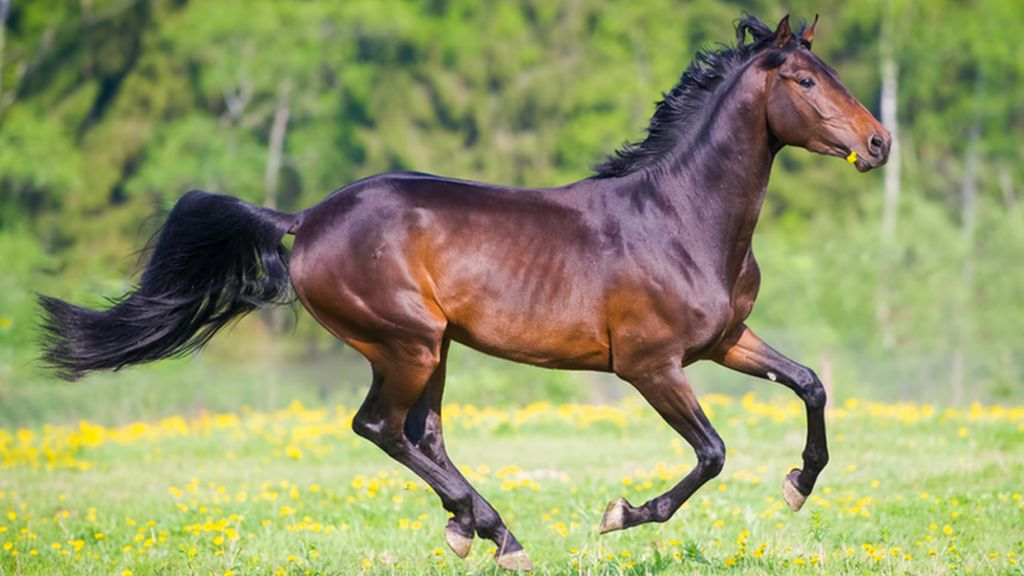
\includegraphics[width=8cm]{horse.png}  % imports graphic as a specified size 
        \caption{A stallion.} % Writes caption below the graphic. 
        \label{fig:horse} % Labels the graphic and allows for cross referencing.
    \end{center} % ends centeing
\end{figure} % ends figure environment
Figure \ref{fig:horse} % cross references the figure labeled horse
shows a horse galloping in a field. This horse looks very similar to my horse named Boe. 

\section{Cool Task } % new section
\subsection{Hyperlinks} % new subsection
One of the ``cool" task I took on was creating hyperlinks within my document. I wanted to be able to link citations to references in the bibliography, as well as create clickable url links. To do so, I used the hyperref package with the arguments colorlink, and I defined the color I wanted to use for urls and citations. 
\subsection{Header} % new subsection
Another cool and useful thing I decided to add to my document was customized header and footer to each page. I used the fancyhdr package, changed the page-style to fancy, used fancyhf command to clear any existing presets for the header, and specified what text I wanted to appear in each cornor of the header; as well as the footer, using the rhead, lhead, and rfoot commands. 

\newpage % creates new page for bibliography
\bibliography{references} % creates bibliography of cited references

\end{document} % ends the document
